\section{Probability of Satisfying Query}
\label{sec:prob_sat}

Now, we have an expression for delay that is built up using random variables for the values of $TF$ and $PL$.  The next useful formulation is providing an expression that describes the probability of a bottleneck flow satisfying its timeliness requirement considering the underlying distributions.  With this formulation, we can define scalability as a network in which the flow's probability of satisfiability exceeds some threshold $P_{thresh}$:
\begin{equation}
	P(D_i < T) \geq P_{thresh}
\end{equation}

Once again, we have our total delay equation of a flow originating in node $i$:
\begin{equation}
	D_i = \frac{ k_{req} \cdot I_S \cdot CF \cdot TF_i}{W} + \frac{P_S \cdot DF \cdot (PL_i-1)}{W}
\end{equation}
Let us define two constants to simplify the expression:
\begin{eqnarray*}
	C_1 = \frac{k_{req} \cdot I_S \cdot CF}{W} \\
	C_2 = \frac{P_S \cdot DF}{W}
\end{eqnarray*}
Then, we can express the delay as
\begin{equation}
	D_i = C_1 \cdot TF_i + C_2 \cdot PL_i
\end{equation}
As we showed in the last section, we can determine $i$ using the expected values for $TF_i$ and $PL_i$, so assuming that we adopt this value of $i$, we can drop the notation:
\begin{equation}
	D = C_1 \cdot TF + C_2 \cdot PL
\end{equation}

\begin{eqnarray}
\nonumber
	f_{TF}^i (tf) = &&\frac{i}{N} \cdot \mathcal{N}(\mu(i),\sigma(i))  \\ \nonumber
			   &+& \sum\limits_{k=i}^{\frac{N}{2}-1} \cdot \frac{\frac{1}{2}-\frac{i}{N}}{\frac{N}{2} - i}\mathcal{N}(\mu(k),\sigma(k))  \\
			   &+& \frac{1}{2} \cdot \mathcal{N} (\mu(\frac{N}{2}),\sigma(\frac{N}{2}))
\label{eq:full_PDF_TF}
\end{eqnarray}











%\begin{figure}
%\begin{centering}
%    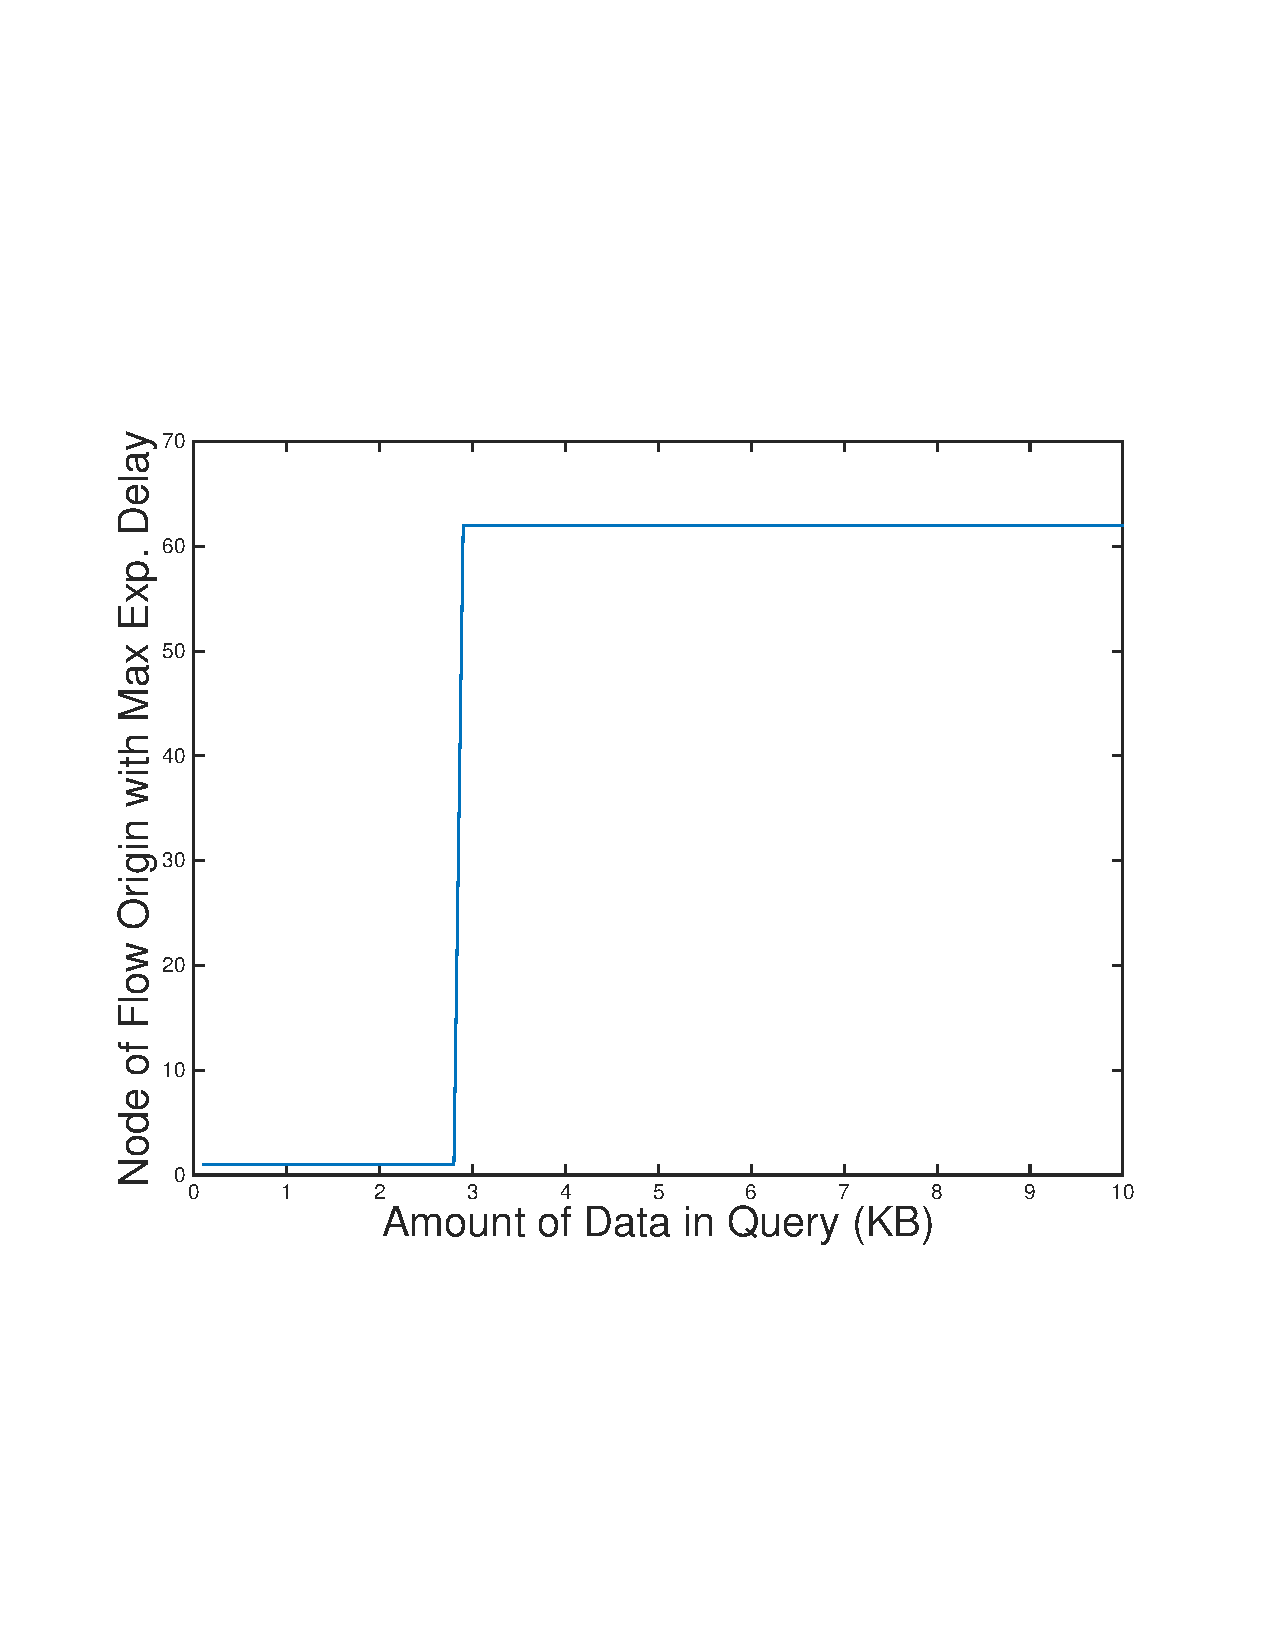
\includegraphics[scale=0.4, clip=true, trim=15mm 65mm 20mm 65mm]{figures/max_i_line_net_125.pdf}
%    \caption{The value of $i$ (origin of a flow) that causes the maximum expected delay.}
%    \label{fig:max_i_line_net}
%\end{centering}
%\end{figure}


